% Para facilitar a manutenção é sempre melhore criar um arquivo por capitulo, para exemplo isso não é necessário 

%---------------------------------------------------------------------------------------

\chapter[Desenvolvimento do Projeto]{Desenvolvimento do Projeto}
Neste capítulo, o desenvolvimento projeto será explicitado e comentado. Por conta a metodologia de desenvolvimento ágil escolhida, cada Sprint possui uma seção no documento, contendo o que foi realizado nela.

\section{User Stories}
Como descrição das necessidades dos usuários desta aplicação, servindo como casos de uso + requisitos funcionais, as seguintes User Storie foram discutidas e, ao longo do projeto, implementadas:

\begin{itemize}
\item Eu, enquanto usuário, devo conseguir cadastrar/logar via Steam Account para usufruir das 
funcionalidades do site.

\item Eu, enquanto usuário, devo conseguir depositar minhas Skins de CSGO do inventário da Steam no 
inventário do Site, a fim de investir nelas no site.

\item Eu, enquanto usuário, devo conseguir depositar apenas as Skins permitidas pelo site, já que o 
site limita as Skins aceitas.

\item Eu, enquanto usuário, devo conseguir colocar na bolsa uma Skins do meu inventário do site, para 
que ela possa valorizar/desvalorizar com o tempo.

\item Eu, enquanto usuário, não posso "sacar" as Skins em investimento no site, apenas as que estão no 
meu inventário.

\item Eu, enquanto usuário, só poderei retornar uma Skins do investimento para o inventário após 1 mês 
de investimento.

\item Eu, enquanto usuário, devo conseguir "sacar" as Skins que estão no inventário do site para o meu 
inventário Steam, para que possa utilizá-las no jogo e na Steam.

\item Eu, enquanto usuário, devo conseguir ver meu histórico de vendas/compras no site, visualizando o 
item comprado/vendido, o preço e a data da compra.

\item Eu, enquanto usuário, poderei ver a valorização/desvalorização das Skins investidas no site, para 
que eu possa saber a hora de comprar e vender.

\item Eu, enquanto usuário, devo conseguir comprar Skins investidas no site com dinheiro.
\end{itemize}

Para maiores detalhes, os cenários de cada User Story foram levantados e anexados ao Apêndice A.

\section{1$^{\circ}$ Sprint}
O primeiro sprint consistiu na preparação do repositório do projeto, com a instalação dos seguintes
FrameWorks: Code Climate, Cucumber, Jest, Travis CI. Além da configuração dessas ferramentas,
foi desenvolvido o primeiro esboço do projeto do projeto para inserção no Heroku e teste da configuração.
Neste esboço, foi criado a Home do site e o arquivo node.js principal. Para a parte de ES4A4,
foi criado o projeto no PivotalTracker, a fim de inserirmos as User Stories.

\subsection{Criação do Repositório no Git}
O primeiro passo tomado pela equipe foi a criação do repositório no Git. Para isso, o integrantes
Guilherme Leão criou o repositório no GitHub, como mostra a figura~\ref{fig:github}, e posteriormente adicionou todos os membros
da equipe e o professor de ES4A4, Daniel Morais.\\
\begin{figure}[!htb]
	\centering
	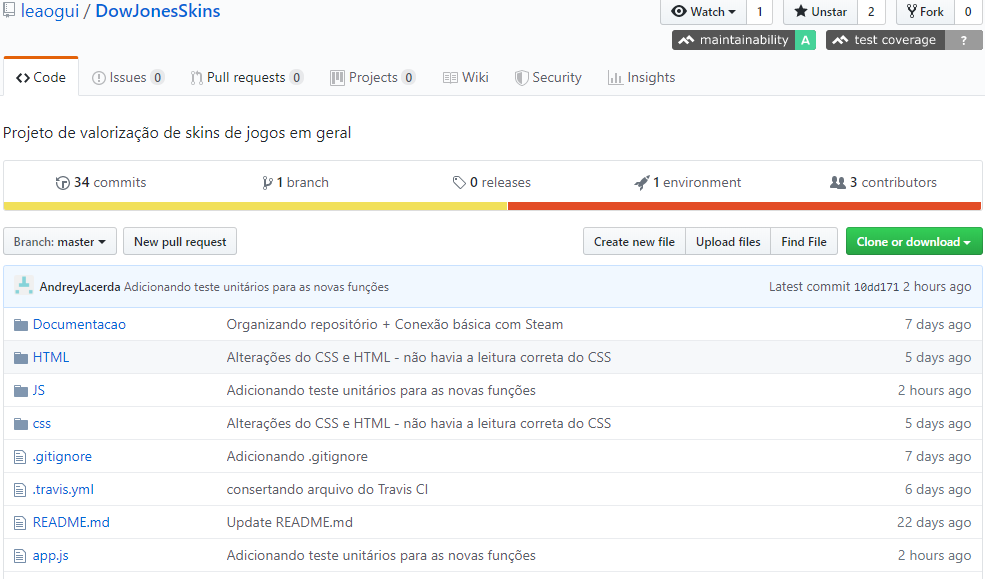
\includegraphics[scale=0.6]{Imagens/Repositorio.png}
	\caption{Repositório do Projeto no GitHub}
	\label{fig:github}
\end{figure}

\subsection{Instalação dos Frameworks}
Dentro da pasta raíz do projeto, o comando 'npm init' foi executado via CMD. Para isso, o Node.js foi instalado
nas máquinas dos integrantes do projeto. Este comando criou três arquivos: node\_modules, que consiste no diretório onde todos
os módulos e bibliotecas utilizadas são salvas; package.json, que consiste em um 'arquivo de configuração',
possuindo informações sobre a execução do project; package-lock.json, que consiste em um arquivo que salva
informações de todas as biliotecas e dependencias instaladas no projeto.

Com esses três arquivos criados, o Jest foi instalado, a partir do comando 'npm install jest', e o Cucumber, a partir
do comando 'npm install cucumber'. Ambos os frameworks são utilizados para testes.

Após a instalação dos dois frameworks para o node.js, os dois frameworks foram instalados para o próprio repositório do GitHub.
O primeiro foi o CodeClimate. Para isso, o dono do repositório instalou a extensão CodeClimate no navegador,
e posteriormente entrou no git do projeto. Dentro do GitHub do projeto, uma opção apareceu para adicionar
o projeto ao CodeClimate. Após clicar na opção, o repositório foi lido e adicionado ao CodeClimate, 
que agora é o plugin de avaliação de código do repositório.

Após isso, o dono do repositório instalou o Travis CI pelo próprio 'GitHub MarketPlace'.

\subsection{Criação e configuração do Heroku}
Para a criação do app no Heroku, o Heroku CLI foi instalado. Com ele instalado, o comando
'heroku create' foi executado via CMD, criando o app no Heroku, como mostra a figura~\ref{fig:heroku}. Após criar o Heroku App, o deploy do Heroku foi configurado
para que ele seja sincronizado com o 'push' para o repositório no GitHub.\\
\begin{figure}[!htb]
	\centering
	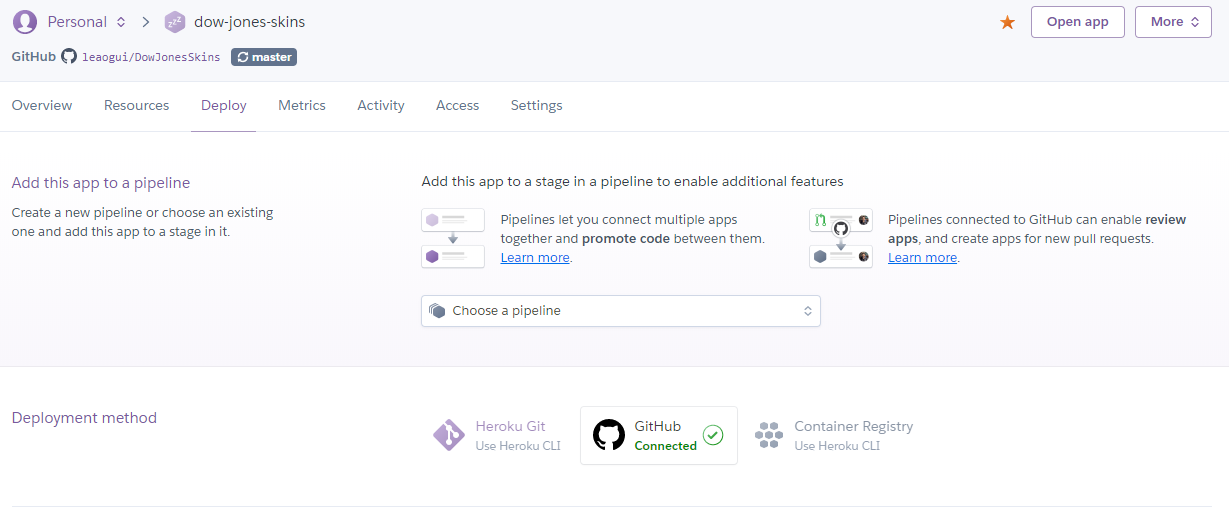
\includegraphics[scale=0.5]{Imagens/Heroku.png}
	\caption{App do Projeto no Heroku}
	\label{fig:heroku}
\end{figure}

\subsection{Home.html + app.js}
Para criar o esboço da Home do projeto, o HTML5 foi utilizado. Para estilização, o Bulma foi explorando,
que consiste num FrameWork de CSS. Cada arquivo foi separado em pastas baseadas em suas extensões. 
Diante disso, uma pasta HTMl, uma CSS e uma JS foram criadas. Na pasta CSS, o .min.css do Bulma foi salvo, para que fosse possível utilizá-lo. A figura~\ref{fig:home} mostra o estado final da construção da primeira 'Home' da aplicação.

Com a Home criada, o próximo passo foi o primeiro contato com o login via Steam. Para isso, a API
da Steam para Node.JS foi utilizada. No arquivos app.js, que consiste no arquivo 'main', todas as rotas foram criadas
e o framework "express" foi utilizado para instanciação do servidor web. Neste arquivo, as rotas da API Steam foram implementadas, configurando
o middleware, informando a API Key e domínio. Por conta da execução ser tanto localmente quanto no Heroku, 
vários arquivos JS com functions fororam modularizados para realizar essa troca de domínio, porta e API Key, já que tais keys mudam para cada domínio (local e Heroku). 

Para essas funções foram criadas testes unitários utilizando o Jest. Esses testes estão na subpasta 'tests' 
dentro da pasta 'JS'.\\

\begin{figure}[!htb]
	\centering
	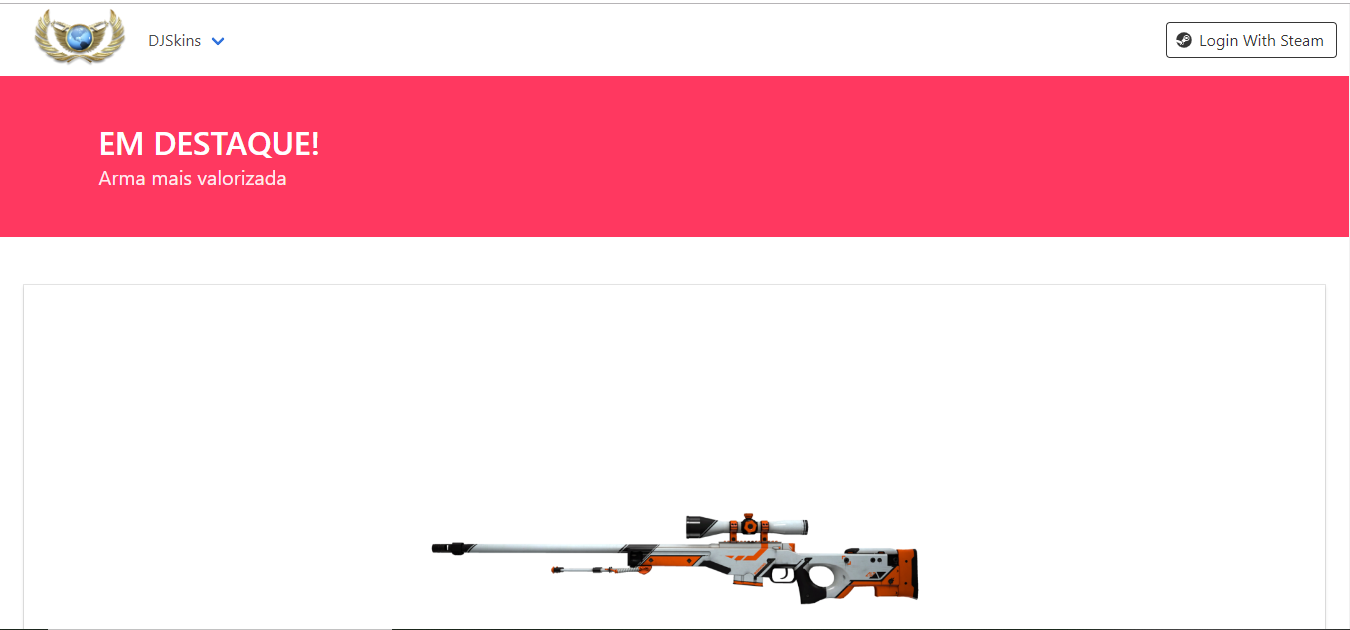
\includegraphics[scale=0.5]{Imagens/Home.png}
	\caption{Esboço da Home pronto}
	\label{fig:home}
\end{figure}

\subsection{Engenharia de Software}
No Pivotal Tracker criado pelo professor Daniel, as primeiras User Stories foram inseridas. Essas Stories consistem 
nas principais funcionalidades de usuários identificadas pelo grupo e divididas até então. Após a inserção, 
Uma pontuação foi atribuída para cada uma, a partir de um debate, onde o integrante que deu a menor nota defendia seu argumento 
junto ao integrante de deu a maior nota. O melhor argumento decide a nota.

Após isso, a prioridade e dependencias de cada User Story foi organizada, além de lançar algumas Users Stories no IceBox, fechando a primeira organização do Pivotal Tracker, como pode ser vista na figura~\ref{fig:pivotal}.\\

\begin{figure}[!htb]
	\centering
	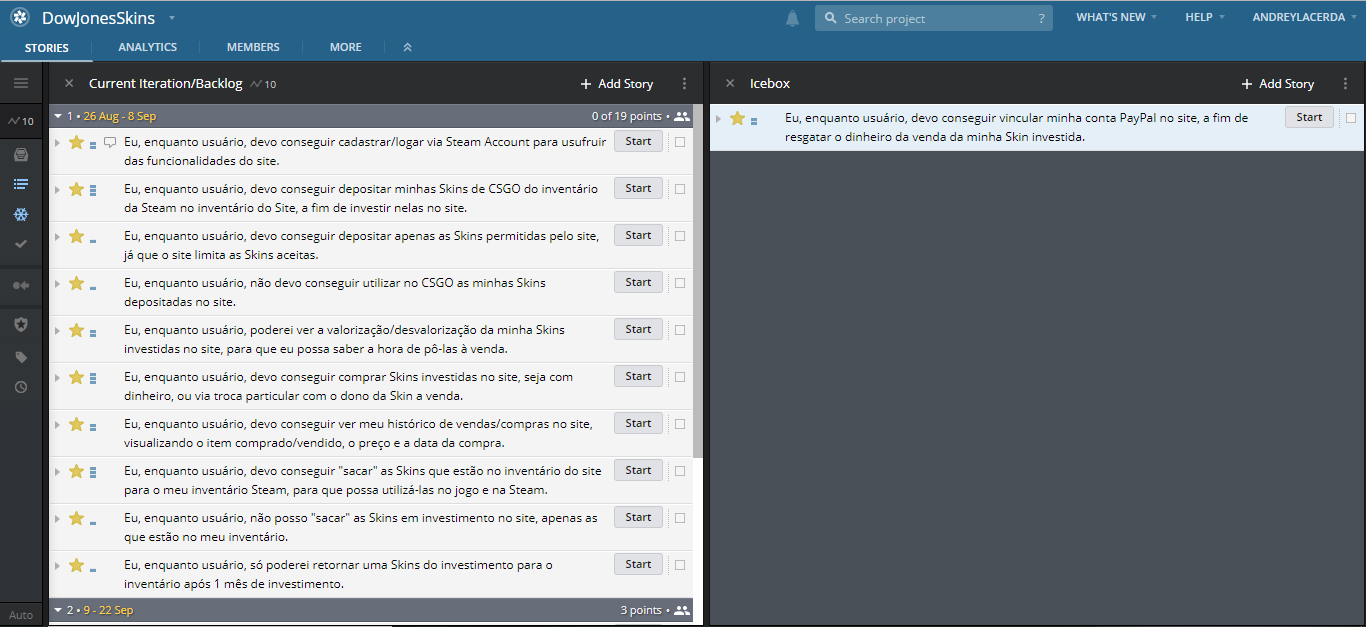
\includegraphics[scale=0.4]{Imagens/Pivotal1.png}
	\caption{PivotalTracker no 1$^{\circ}$ Sprint}
	\label{fig:pivotal}
\end{figure}

\section{2$^{\circ}$ Sprint}
\subsection{Descrevendo as features com Cucumber}
Com as User Stories definidas, o passo seguinte foi esboçar todas as features utilizando o ideal do BDD 
e utilizando o Cucumber para isso. Com isso, os possíveis cenários de todas as User Stories foram descritos até então, seguindo como base o projeto exemplo mostrado pelo professor Daniel, 
mais a própria documentação do Cucumber.

Como Dito anteriormente, para isso a sintaxe do Cucumber foi utilizada, e cada feature foi separada em um arquivo diferente, 
salvas em uma pasta separada, chamada 'Features'. 
Como sintaxe, cada User Storie foi salva como Feature, com suas descrições, Backgrounds, e assim Cenários.

\subsection{Testando cadastro/login com PostgreSQL do Heroku}
Para começar o sistema de cadastro/login, o add-ons do PostGre foi adicionado ao Heroku via Heroku CLI. Para isso, 
o comando 'npm install pg' foi utilizado para instalar o Postgres do projeto. Após isso, o add-on do Postgre foi instalado no
Heroku via CMD, com comando 'heroku addons:create heroku-postgresql:hobby-dev'. Após isso, os passos 
que estão na documentação do Heroku Postgre foram seguidos, encontrados em 'https://devcenter.heroku.com/articles/heroku-postgresql'.

Após isso, as tabelas foram criadas via CMD, usando comando 'heroku psql' e adicionando todas as linhas de comando sql.
Tendo a conexão estável e as tabelas criadas, uma classe chamada 'UserCRUD' foi desenvolvida, e nela o JSON 
enviado pela Steam após conexão foi utilizado para salvar um usuário novo no banco de dados.

Nessa classe, a função signUp() recebe o JSON da Steam, conecta ao banco de dados e verifica se este usuário 
já foi cadastro. Se sim, mais nada é feito, mas caso contrário, o usuário é inserido no banco de dados.
Tendo isso feito, a primeira parte do sistema de cadastro/login foi finalizada.

\subsection{Estabelecendo Sessão}
A fim de estabelecer o sistema de login, a utilização de sessão para bloquear o acesso de usuário a 
determinadas páginas do site foi a solução mais viável. Para isso, a constante Session da biblioteca 'Express' foi utilizada.

O comando app.use() foi utilizado para usar o Session. Neste etapa, um id paraa sessão foi inserido dentro do 
parâmetro de inicialização 'secret', e false foi posto nos outros dois itens de inicialização, saveUninitialized e resave, que, 
após pesquisar, foi decidido que não fariam sentido algum.

Após isso, dentro da página '/verify' foi colocada a criação da sessão de acordo com o login do usuário na Steam. 
Com o usuário autenticado via Steam, o comando 'req.session.user' foi itilizado e o JSON fornecido pela Steam 
foi atribuído à essa constante.

Com isso, uma sessão é criada para cada usuário logado, e após isso, para bloquear o acesso à páginas sem que o user 
esteja logado, um 'IF' foi inserido em cada get do servidor (ignorando a /index e a /login). Dentro do IF, 
'!req.session.user' foi inserido, mostrando que caso não exista ression, o usuário deveria ser redirecionado para a 
tela de login da Steam, finalizando assim o ideal de sessão do site. 

\subsection{Visualizando o inventário Steam do usário}
Para obter acesso ao inventário Steam do usário logado, a biblioteca 'steam-inventory-api' foi utilizada. 
O serviço da API é inicializado quando o servidor sobe. Após isso, ao se loga na Steam, o usuário é redirecionado para o '/verify' onde, 
além de ter a sessão instanciada, os itens de seu inventário são visualizados.

Para isso, a steamId do usuário de dentro do JSON fornecido pela Steam foi recuperada e inserida como um dos diversos parâmetros da API de 
inventário. Constantes foram utilizadas para facilitar o preenchimentos dos outros parâmetros de inicialização, seguindo como base o 
exemplo de uso da API fornecido em 'https://www.npmjs.com/package/steam-inventory-api'.

Com isso, ao logar no Steam, o sistema consegue capturar todos os itens trocáveis do inventário do usário, 
além de filtrar para o jogo 'CSGO'.


\section{3$^{\circ}$ Sprint}
\subsection{Personalização via Cookie}
A fim personalizar a tela do usuário logado, cookies foram utilizados para 
exibir seu avatar e seu username. Para isso, o JSON disponibilizado pela steam logo 
após a autenticação do usuário é salvo no cookie e posteriormente resgatado por duas 
funções JavaScript encarregadas de resgatar o avatar e o username do user.

Com isso, o avatar do usuário foi printado na navbar de todas as telas, enquanto logado, enquanto seu nome 
aparece na página 'Minha Conta'.

\subsection{Template Engine Handlebars}
Conforme o projeto foi evoluindo, sua complexidade foi aparecendo. Sabendo que seria necessário o retorno 
de muita informação do banco de dados para a tela da aplicação, além de muitas regras que resultariam 
em manipulação do banco, tornou-se necessária a utilização de um Template Engine, tornando a aplicação 
inteiramente back-end. 

Diante disso, o ‘Handlebars’ foi instalado no sistema e marcado como template engine. Após isso, todos 
os HTMls desenvolvidos até então foram trocados para Handlebars, e as devidas alterações no back-end 
foram realizadas.

O HBS foi a escolha por conta de sua natureza totalmente virada para o Node.js, o qual foi utilizado 
para o back-end inteiro, e por conta de seu fácil aprendizado e resultado que solucionaria os 
problemas do projeto.

\section{4$^{\circ}$ Sprint}
\subsection{Mecânica de Depósito e Saque de Skins}
A fim de criar a mecânica de deposito e saque de skins, a API ‘steam-inventory’ foi utilizada, 
junto a algumas funções próprias.

Ao acessar o próprio inventário do DJS, a API ‘steam-inventory’ é utilizada, retornando todas as 
skins trocáveis de Counter-Strike: Global Offensive. Com essa informação, o nome de tais skins são 
printadas na tela do usuário em uma coluna a esquerda da tela, enquanto apenas as aceitadas pelo site 
são printadas na coluna do meio. Na coluna a direita, por sua vez, foi utilizada para printar as 
skins já depositadas no site pelo usuário. 

Com todas as informações na tela, botões foram adicionados. Na coluna do meio, botões que chamam 
uma função para investir a skin clicada foram adicionados, enquanto na coluna a direita, botões 
para sacar skin e investir na skin foram adicionados. A coluna a esquerda ficou apenas com nomes 
de skins.

Os botões chamam funções, que por sua vez, realizam as devias validações e manipulações no banco 
de dados, possibilitando assim o mecanismo de deposito e saque.

Devido a burocracias com a Steam, não foi possível criar uma conta para realizar as trocas reais 
de skins. Com isso, ao depositar uma skin, tal skin não some do inventário real do usuário, 
apenas é mapeado para dentro do inventário do DJS. A mesma coisa para o saque, em que a 
skin é realmente enviada para a Steam, mas sim apenas retirada do inventário do DJS, 
simulando tal troca.

\subsection{Mecânica de Investimento de Skins}
A fim de investir na skin, mecanismo core da aplicação, o botão na ‘Investir’ foi criado 
para cada skin no inventário DJS do usuário. Ao clicar no botão, uma função é invocada, 
que realiza a confirmação do investimento da skin, marcando a data do investimento.
Com a data marcada, o usuário não pode retirar o investimento até bater 31 dias, que 
consiste em outro User Story do projeto.

A fim de simular a flutuação de valores das skins do mercado, ao investir em uma skin, 
caso a skin investida é a primeira no sistema inteiro, seu valor aumenta 
15\%. Caso contrário, cai 3\%.

\section{5$^{\circ}$ Sprint}
\subsection{Mecânica de Carteira}
Após a implementação do deposito, saque e investimento de skins, a mecânica de carteira foi 
desenvolvida para possibilitar a compra de skins. Para isso, foi criado uma sessão ‘Carteira’, e 
uma coluna ‘saldo’ na tabela ‘usuario’ do Postgresql. 

Ao clicar em ‘Depositar’ na sessão de ‘Carteira’, automaticamente R\$15 creditados em seu ‘saldo’, 
realizando um UPDATE no banco de dados. Ao informar uma quantia a sacar e clicar em ‘Retirar’, tal 
quantia é validada com o saldo. Se o saldo for maior ou igual a quantia, tal valor é debitado do 
saldo, realizando outro UPDATE no banco de dados.

\subsection{Mecânica de Compra de Skins e Histórico de Vendas}
Para o mecanismo de compra, foi criado a sessão ‘DayTrade’, em que o usuário 
acessará para ver todas as skins investidas no site e seu determinado preço, além 
de ver seus próprios investimentos, possibilitando o cancelamento de algum deles, 
caso tenham mais de 31 dias.

Com isso, ao encontrar um skin que deseja, o usuário clica em ‘Comprar’, e uma função é 
chamada para validar a compra. Se a compra for válida, o usuário comprador recebe a skin 
do usuário “vendedor” que está a mais tempo com o investimento aberto. Com isso, do saldo do 
comprador é debitado o valor da skin, enquanto do saldo do vendedor é creditado tal valor. 

Além disso, um histórico de vendas é criado, marcando assim o nome do vendedor/comprador, as 
informações da skin comprada e a data da compra. Tal histórico também pode ser visto na tela 
‘DayTrade’.

\subsection{Testes}
Após todos os desenvolvimentos serem concluídos e testados pela equipe, o desenvolvimento de 
teste automatizados foram realizados. Para isso, o framework de testes Jest foi utilizado para 
o testes unitários e de integração, enquanto o Puppeteer e o Cucumber foram utilizados para os 
testes End-To-End. 

Ao total, dezesseis testes foram implementados, testando as funcionalidades principais do sistema, 
evitando qualquer má manipulação de banco de dados e interferência no mecanismo de valorização de
skins do site.

Além desses testes, uma ferramenta de análise estática foi utilizada no projeto. Tal ferramenta 
foi o ‘jshint’, e serviu como “cleaner” de “code smells”. A análise estática de 100\% ao final 
das refatorações requisitadas pela ferramenta.

%\section{Tipo de Pesquisa}
%\lipsum[3-5]

%\section{Plano Amostral (se Pesquisa Quantitativa)}
%\lipsum[3-5]

%\section{Instrumento de Pesquisa e Escalas Utilizadas (Escalas se Pesquisa Quantitativa)}
%\lipsum[3-5]

%\section{Coleta de Dados}
%\lipsum[3-5]

%\section{Análise de Dados}
%\lipsum[3-5]


%---------------------------------------------------------------------------------------


%---------------------------------------------------------------------------------------
%\chapter{Considerações finais}
%\lipsum[3]

%\section{Resposta à Questão de Pesquisa}
%\lipsum[3-5]

%\section{Objetivos Propostos}
%\lipsum[3-5]

%\section{Contribuições Academicas e Gerenciais}
%\lipsum[3-5]

%\section{Limitações da Pesquisa e Contribuições para Estudo}
%\lipsum[3-5]




